\documentclass{article}
\usepackage{tikz}
\usepackage[paperwidth=21cm, paperheight=29.7cm, top=4.85cm, bottom=4.85cm, left=0.5cm, right=0.5cm]{geometry}

\pagestyle{empty} % remove numeração de página

\setlength{\parindent}{0pt} % remove indentação
\setlength{\parskip}{0pt}   % remove espaçamento entre parágrafos

\begin{document}
\vspace*{-4.85cm} % remove espaço que empurra pra segunda página

\begin{center}
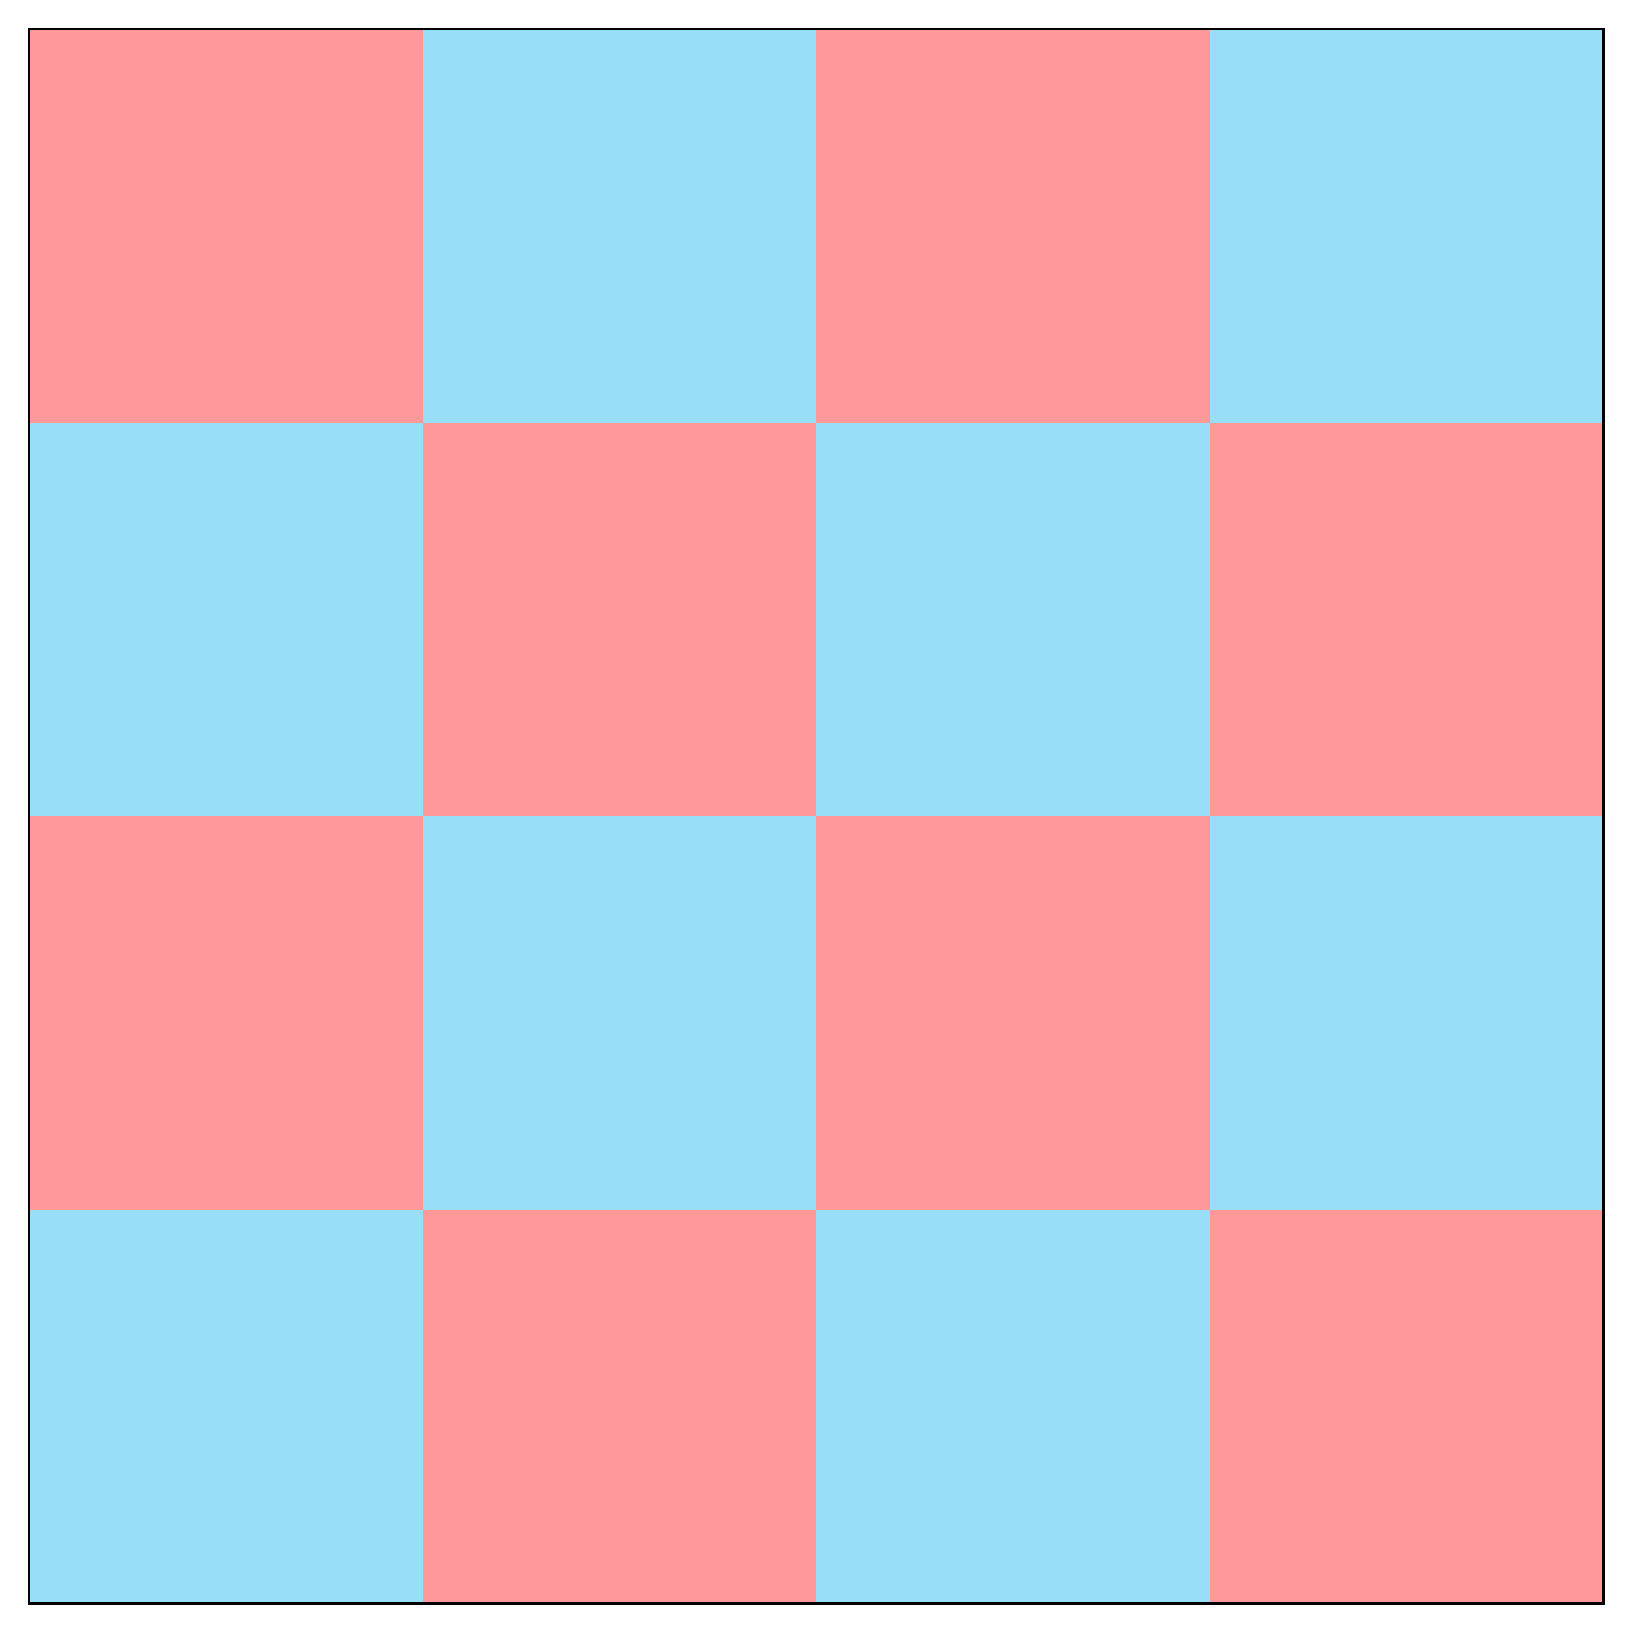
\begin{tikzpicture}
  \def\squareSize{5} % em centímetros

  \foreach \row in {0,1,2,3} {
    \foreach \col in {0,1,2,3} {
      %\pgfmathparse{mod(\row+\col,2) == 0 ? "brown!50!yellow" : "green!50!black"}
	  %\pgfmathparse{mod(\row+\col,2) == 0 ? "cyan!30!white" : "blue!70!black"}
	  %\pgfmathparse{mod(\row+\col,2) == 0 ? "olive!30!yellow" : "olive!80!black"}
	  %\pgfmathparse{mod(\row+\col,2) == 0 ? "orange!40!white" : "brown!80!red"}
	  %\pgfmathparse{mod(\row+\col,2) == 0 ? "gray!20!cyan" : "blue!80!gray"}
	  %\pgfmathparse{mod(\row+\col,2) == 0 ? "red!80!yellow" : "cyan!70!blue"}
	  %\pgfmathparse{mod(\row+\col,2) == 0 ? "orange!80!yellow" : "purple!70!black"}
	  %\pgfmathparse{mod(\row+\col,2) == 0 ? "lime!80!green" : "magenta!70!purple"}
	  \pgfmathparse{mod(\row+\col,2) == 0 ? "cyan!40!white" : "pink!80!red"}
      \edef\colorname{\pgfmathresult}
      \fill[\colorname] (\col*\squareSize, \row*\squareSize) rectangle ++(\squareSize, \squareSize);
    }
  }

  \draw[line width=1pt] (0,0) rectangle (20,20);
\end{tikzpicture}
\end{center}

\end{document}
